 \chapter{Model and backgrounds}

 
\section{Signal of Interest}

The model that is going to be study is based on a reciently proposed new mechanism of production of heavy neutrinos through the Higgs Boson decay \cite{Seesaw Mechanism with displaced vertices}. One favourable characteristic of this model is that in a natural escenario the mass of the heavy neutrinos can lie at the electroweak scale. The theoretical study by \cite{Seesaw Mechanism with displaced vertices} propose the experimental search of the heavy neutrinos using a technique known as displaced vertices.

According to this model when the mass of the heavy neutrinos is inferior than the mass of the Higgs, the latter can present novel decay channels. The Higgs boson can decay into a light and a heavy neutrino, followed by a subsequent decay of the heavy neutrino via a charged or neutral current interaction. Then, the decays of the heavy neutrino can be represented by: $N \rightarrow l^+ l^- \nu$ or $N \rightarrow l q q'$. Thus, there are two possible final states of the event of interest: two leptons, two jets (from the VBF process) and $\vec{E_T^{miss}}$ (due to the neutrino) or four jets (two of the VBF process and two from the quarks of the heavy neutrino decays), $\vec{E_T^{miss}}$ and one lepton. The first type of final state is going to be called hadron signal, while the second will be named leptonic signal.

If the heavy neutrino would have a mass of the order of a few GeV, the Higgs and heavy neutrino would travel a certain distance before decaying. Since both particles are not detected, the decay products are expected to have associated tracks with displaced vertices. For this reason, the presence of displaced vertices in the detector is an important signal to prove this model because it could indicates the presence of the heavy neutrino in the detector. Nevertheless, due to in this model the resulting leptons have a low momentum. Thud, due to experimental restrictions of the available triggers in CMS and ATLAS, the theoretical analysis proposed in reference \cite{Seesaw Mechanism with displace vertices} is not achievable.  

The High Energy Physics Group at Universidad de los Andes has proposed a technique that allows to study at the LHC the production of heavy neutrinos through the decay of the Higgs boson. While in the model proposed in \cite{Seesaw Mechanism with displace vertices} consider the production of the Higgs boson through the fusion of two gluons, we consider the Higgs production through two vector bosons fusion. These vector bosons ($W^{\pm},Z^0,\gamma$) come from an interaction process between two quarks. These both quarks belong to protons from opposite beams that will collide in a particle accelerator. The former described process is know as Vector Boson Fusion (VBF) \cite{VBF processes}. 

Finally, as a result of the two vector boson fusion, a Higgs boson is produced and the initial quarks that interacted manifest themselves as jets with high transverse momentum in the opposite hemispheres of the detector. For this reason, in Experimental Particle Collider Physics the events in which two jets of high transverse momentum are detected located at opposited hemispheres of the detector and with a high separation of pseudorapidity are labeled as candidates of processes of VBF. The feynman diagram ilustrating the process already described in which just one lepton is produced is showed in figure....

\begin{figure}[h] \label{Signal_feynman}
\centering
\caption{Feynman diagram for the hadronic signal}
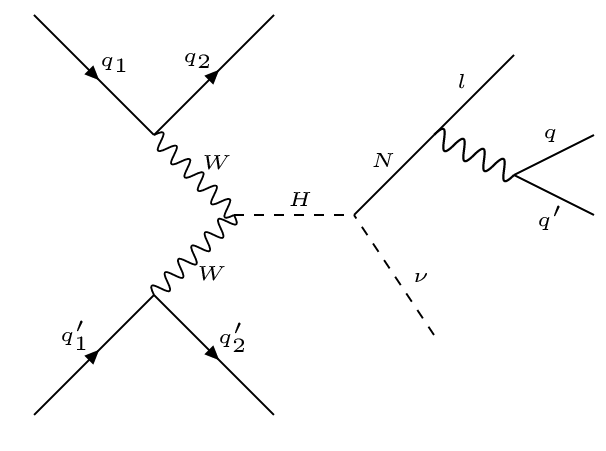
\includegraphics[width=0.6\textwidth]{./Capitulos/Model/signal}  
\end{figure}

%The observation of the Higgs decay into heavy neutrinos would be a firm prove of the Type I Seesaw mechanism \cite{Type I Seesaw Mechanism}. The former would prove the existence of physics beyond the SM associated to the mass of the neutrinos.
 
 
 \section{Backgrounds}
 
The main problem of detecting an event of interest is that the magnitude of its signal is significantly smaller with respect to some processes from the SM. For this reason, the processes from the SM that have the same or similar final states as the signal are called backgrounds. Thus, it is fundamental to develop procedures in order to reduce the experimental background under the magnitude of the searched signal. These procedures usually use different variables that exploit the topology of the event and its kinematic characteristics. For example, one of the most famous variables is missing transverse energy ($\vec{E_T^{miss}}$), it is defined as the minus sum of the transverse momentum of the particles that are detected (visible particles). When a set of variables that potentially separate the signal from the background is determined, it is necessary to find the optimal values of them that allow to reduce as much as possible the background. 
 
 \subsection{W + Jets Background}
  
 \subsection{Drell Yan + Jets Background}
 
 \subsection{$t \bar{t}$ Background}
 
 